\chapter{Real-time planlægning}
Vi vil i dette kapitel beskrive Real-time planlægning (RTP), samt diskutere hvordan det kan implementeres i \pycsp. 

RTP er baseret på den kendsgerning at nogle begivenheder i programmer kan være vigtigere at få udført end andre indenfor en afgrænset tidsperiode. Dette kan f.eks. være interrupts, input- eller output enheder eller interne processer. Med RTP tilknytter man en deadline for hver begivenhed, som bruges til at planlægge rækkefølgen for afvikling af begivenhederne. Formålet er at optimere antallet af begivenheder der når at blive udført inden deres deadline er overskredet. Normalt anses alle begivenheder for at være lige vigtige, og de planlægges ud fra en optimal udnyttelse af processoren. Denne optimale processorudnyttelse kan man være nødt til at gå på kompromis med hvis man ønsker at bruge RTP og derved prioritere visse begivenheder højere end andre. Man kan forestille sig en situation hvor man ikke starter en begivenhed med lav prioritet selv om den er klar, hvis man ved at en begivenhed med høj prioritet er klar kort tid efter, og venter derfor på at den er klar og igangsætter begivenheden med høj prioritet med det samme. 
RTP benyttes meget i specialiserede indlejrede systemer til f.eks medicinsk udstyr, kontrol af luftrummet, på rumstationen ISS\cite{Audsley1990} og mange andre steder. Det er dog også anvendeligt i i mere gængse applikationer, typisk i forbindelse med en eller anden form for interaktion med den virkelige verden. 

I litteraturen omkring RTP bruges begreberne hard- og soft deadlines samt hard- og soft real-time systemer forskelligt, så vi vil i det følgende gennemgå hvordan vi definerer disse begreber. Vi har valgt at illustrere deadlines ved hjælp af time-value funktioner, hvor "værdien" indikerer det bidrag begivenheden bidrager med til systemets overordnede mål. 

\subsubsection{Kritisk deadline}
En kritisk deadline er en deadline som under alle omstændigheder skal overholdes for at opretholde systemets integritet. Såfremt en kritisk deadline overskrides vil der påføres skader på systemet som kan forårsage at systemets tilstand bliver udefineret. En kritisk deadline er illusteret i \cref{fig:hard-rtp}.

\begin{figure}
 \begin{center}
  
\includegraphics[scale=0.75]{images/critical-deadline}
	\caption{Begivenhed med kritisk deadline.}
	\label{fig:hard-rtp}
\end{center}
\end{figure}


\subsubsection{Hard deadline}
Vi definerer en begivenhed til at have en hard deadline såfremt en færdiggørelse af begivenheden efter deadlinen ikke tilfører systemet nogen positiv værdi. Modsat en kritisk deadline kan en overskridelse af en hard deadline accepteres. I \cref{fig:hard-dl} vises en hard deadline for en begivenhed. 

\begin{figure}
 \begin{center}
  
\includegraphics[scale=0.75]{images/hard-deadline}
	\caption{Begivenhed med hard deadline.}
	\label{fig:hard-dl}
\end{center}
\end{figure}
%Her tilføres der en positiv værdi til programmet hvis begivenheden afsluttes mellem dens starttidspunkt og dens deadline. Hvis begivenheden først er færdig efter deadline har den ingen værdi. En soft deadline (\cref{figure:soft-dl}) tilføjer den samme værdi som en hard deadline hvis begivenheden bliver færdig rettidigt. 

\subsubsection{Soft deadline}
Færdiggørelse af en begivenhed med en soft deadline til tiden tilføjer samme værdi til systemet som hvis den havde haft en hard deadline. Forskellen ligger i den tilførte værdi såfrem deadlinen overskrides. Hvor en hard deadline ikke tilføjer nogen værdi ved en overskridelse, vil en overskridelse af en soft deadline stadig tilføre en reduceret værdi ved færdiggørelse. Den tilførte værdi vil være omvendt proportional med længden af overskridelsen. \cref{figure:soft-dl} illustrerer en soft deadline. 

\begin{figure}
 \begin{center}
  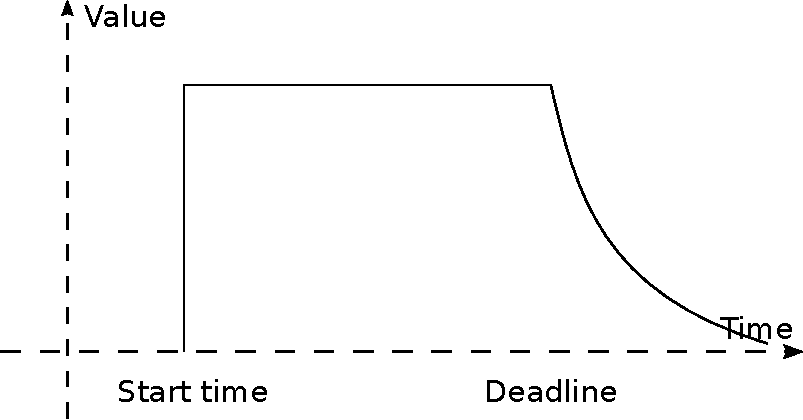
\includegraphics[scale=0.75]{images/soft-deadline}
	\caption{Begivenheden med soft deadline.}
	\label{figure:soft-dl}
\end{center}
\end{figure}


%Hvis deadlinen overskrides mindskes værdien den begivenhed tilføjer, omvendt propotionalt med overskridelsen. Ved en hard deadline er der ikke tilknyttet en egentligt %straf hvis en begivenhed ikke overholder sin deadline. Dette er derimod tilfældet i \cref{fig:hard-rtp}, der viser en begivenhed der tilføjer negativ værdi ved overtrædelse af en deadline. Hvis den tilknyttede straf for ikke at overholde en deadline er større end en hvad programmet maksimalt kan opnå ved at overholde alle deadlines kaldes det et ``hard real-time system''\cite{Laprie1989}.

\subsubsection{Hard real-time system}
Et hard real-time system er defineret ved et system der har begivenheder med hard deadlines, og kan garantere at disse ikke overskrides. Ydermere skal systemet være derterministisk, så denne garanti kan gives på forhånd. Det giver ikke mening at snakke om kritiske deadlines i hard realtime systemer da de kun adskiller sig fra hard deadlines med henblik på konsekvensen af en overskreden deadline, hvilket per definition ikke må ske i et hard real-time system.  

\subsubsection{Soft real-time system}
Et soft real-time system kan indeholde alle typer deadlines men opstiller ikke nogen garantier for at de overholdes. Det vil typisk bruge en algoritme til at op- og nedprioritere hvilke deadlines der skal overholdes såfremt alle deadlines ikke kan overholdes.\\
\\

Generelt vil der i et real-time system ikke være alle begivenheder der har den samme type af deadline. Nogle begivenheder har ingen deadline, nogle har en soft deadline, og få har en hard eller eventuelt en kritisk deadline. 
%For RTP skal kørslen planlægges så begivenhederne har den maksimale udnyttelse af tilgængelige ressourcer samtidigt med at så mange deadlines som muligt overholdes, hvor de vigtigte deadlines prioriteres højest. 

\section{Planlægning af begivenheder}
Planlægningen af hvilke begivenheder der skal køres hvornår, tager udgangspunkt i det overordnede formål med systemet. Generelt vil formålet være at minimere antallet af overskredne deadlines, men dette er sjældent det eneste kriterie der planlægges efter, ofte vil prioriteten for, og tiden det tager at udføre en begivenhed indgå i planlægningen. Eksempelvis vil man ofte prioritere at nå en kritisk deadline selv om det betyder at man overskrider to soft deadlines. 

%De fleste eksisterende real-time systemer arbejder på isolerede systemer, hvor planlæggeren har fuld kontrol over hele computeren. Derfor er hovedparten af forskningen indefor området gået til udarbejdelsen af specialiserede kerner og komplette operativsystemer\cite{damm1989real, jones1979staros, levi1989maruti,ramamritham14scheduling}. Vi ønsker i modsætning hertil ikke at udvikle en specialiseret kerne, men lade \sched en i \pycsp kunne planlægge processer efter bedste evne baseret på informationer den har om processerne.

For at foretage en planlægning af begivenheder der opfylder systemets formål bedst muligt, skal vi have så meget information om begivenheder som muligt - jo mere vi ved om dem jo bedre en planlægning kan der foretages. De relevante informationer i forhold til planlægningen er, hvornår en begivenhed forekommer, hvor lang tid den tager at udføre samt hvilken prioritet den har. 

Ud fra den tilgængelige viden kan der foretages en statisk eller dynamisk planlægning\cite{cheng1987scheduling}. Statisk RTP kræver at vi har alle de nævnte informationer om alle begivenheder. Herved kan vi på forhånd foretage en fuldstændig planlægning og allerede inden start have klarlagt om nogen deadlines vil blive overskredet. Såfremt vi ikke har alle informationer til rådighed, er vi nødsaget til at foretage en dynamisk planlægning. Dette vil ofte skyldes at vi enten ikke ved hvornår en begivenhed forekommer, eller at vi ikke har information om hvor lang tid der tager at udføre en begivenhed. I praksis vil det være svært at opstille eksakte værdier for hvor længe en begivenhed er om at blive udført og der benyttes derfor ofte estimater i stedet for. \fxnote{hvilken betydning har det at der benyttes estimater i stedet for eksakte værdier?}

%Overordnet kan begivenheder planlægges enten statisk eller dynamisk\cite{cheng1987scheduling}. I statisk RTP er alle begivenheder kendt på forhånd. Planlæggeren kan i dette tilfælde allerede inden start udregne om det er muligt at overholde alle deadlines. Alternativt planlægges begivenhederne dynamisk hvis der uregelmæssigt kan ankomme nye begivenheder der skal planlægges. 

%\fxnote{Motivationen her skal være at vi skal kende begivenheders frekvens og længde - skriv noget om det!}
%I realtidssystemer er næsten alle begivenheder cykliske, med enten en regelmæssig eller tilfældig frekvens. Begivenheder der forekommer med en regelmæssig frekevens kan være f.eks. være målinger der skal foretages med bestemte intervaller, hvor uregelmæssig frekvens ofte vil være tilfældet ved begivenheder der skal indtræffe som reaktion på udefrakommende input, f.eks. fejl eller alarmer. 

%\begin{shaded}
%Til planlægningen har planlæggeren behov for at vide hvor lang tid det vil tage at udføre en given begivenhed per periode, men da dette tal enten ikke er kendt eller fast for hver periode, bruges der ofte estimater. Dette medfører at en aperiodisk begivenhed kan ankomme på et vilkårligt tidspunkt og da planlæggeren kun har et estimat for tidsforbruget kan man  ikke tilknytte en ``hard deadline'' til aperiodiske begivenheder, da der altid findes en kæde af aperiodiske begivenheder der medfører en overskridelse af en deadline. 
%\end{shaded}

%\fxnote*{Dette skal måske flyttes eller omformuleres så vi ikke med det samme begrænses til dynamiske \sched}{I \pycsp kan der til alle tidspunkter tilføjes nye processer, og derfor vil vi kun beskæftige os med en dynamisk \sched. Desuden har man ikke med \pycsp fuld kontrol over hele operativsystemet. Mængden af processerkraft vi har til rådighed til kørsel af processerne vil derfor varriere uafhængigt af \pycsp, hvorfor vi heller ikke kan lave et pålidelig ``hard real-time system'', men fokusere på et ``soft real-time system''.}

\subsection{Metoder til skemaplanlægning}
Der findes adskillige metoder til at planlægge rækkefølgen af begivenheder. De adskiller sig fra hinanden med henblik på hvilke informationer der er til rådighed og hvad de optimerer efter. Vi har valgt at kigge på ``Rate monotonic algorithm''\cite{lehoczky1989rate,liu1973scheduling} og ``Earliest deadline first''\cite{liu1973scheduling} indenfor henholdsvis statisk og dynamisk skemaplanlægning.

Hvor processer isoleret set har behov for at udføre deres opgave inden deres deadline, har \sched en behov for kvantitativt at kunne organisere dem indbyrdes, således den til enhver tid kan vælge hvilken proces der skal udføres som den næste. Hovedformålet for en  \sched ~ er derfor at gå fra en række processer med tilknyttet deadline og eventuelt andre egenskaber til en prioriteret liste. \\
Der fokuseres i litteraturen på om en algoritme er stabil eller ej. Såfremt en algoritme er stabil vil man kunne definere en delmægnde af begivenheder, for hvilke man kan garanterer at de ikke overskrider deres deadline. 

\subsubsection{Rate monotonic algorithm (RM)}
RM er en statisk \sched, der fra start af udregner en prioriteret liste på baggrund af frekvensen af processens periode, dermed vil processer der oftet skal have udført deres periode en højere prioritet, end processer med lav frekvens. RM er todelt og i første del udføres før selve simuleringen udregnes  prioriteten for processerne, og udvælger hvilke processer der kan medtages i selve udførslen. Anden del står for udvælgelsen af processer  under simuleringen, og her vælges simpelt den proces med den højeste prioritet. 

Et problem for RM er at ved udvælgelsen af processer der kan medtages har man ikke en optimal udnyttelsen af processorkraft. \Citeauthor{lehoczky1989rate} er kommet frem til at ``worst-case'' er udnyttelsen i gennemsnit 88\\cite{lehoczky1989rate}. Et større problem i relation til implementering i \pycsp er dog at RM er dog at den er statisk. Til gengæld er algoritmen stabil ved en overskridelse af deadline for en proces. 

\subsubsection{Earliest deadline first (EDF)}
Som alternativ til den statiske \sched, hvor man ikke kan ændre prioriten af processen løbende gennem simuleringe, findes de dynamiske \sched er, hvor er EDF er et eksempel. Her evalueres prioriterne af processerne dynamisk igennem simuleringen og evaluere dermed løbende hvilke processer der skal udvælges. I EDF har den proces hvis deadline ligger tættest på højest prioritet og den hvis proces har længst til deadline den laveste prioritet. Aperiodiske processer kan i EDF indgå på lige fod med de periodiske da man til hvert processkift evaluere hvilken der har den nærmeste deadline, som både kan være en periodisk proces som en aperiodisk.

Udnyttelsen af processorkraft kan i EDF komme op på 100\, da alle processer bliver planlagt løbende i modsætning til RM der foretager et valg om en given proces kan planlægges.  Ulempen ved EDF er den ikke er stabil i det vi ikke har kontrol over hvilke processers deadline der bliver overskredet. Dette er specielt et problem hvis man har en en uhomogen samling processer hvor en mindre del er kritiske.

\subsubsection{Least Laxity(LL)}
LL er en modifikation af EDF. LL kigger på hvor lang tid en begivenhed tager at udføre sammenholdt med hvor lang tid der er til deadline for begivenheden. Laxity er defineret som deadline minus tiden det tager at udføre begivenheden. Laxity bliver altså et udtryk for hvor presserende det er at igangsætte en begivenhed for at den kan nå sin deadline. I LL bruges dette til at prioritere de begivenheder der har mindst laxity højest når begivenhederne planlægges. \\
\\
I systemer hvor begivenheder ikke er isolerede men kan have interne afhængigheder, kan der opstå det problem der hedder prioritetsinvertering\cite{sha1990priority}. Dette problem opstår hvis en begivenhed med høj prioritet er afhængig af en begivenhed med en lavere prioritet. Derved bliver begivenheden i praksis kørt med den lavere prioritet da den ikke er klar før begivenheden med lav prioritet er færdig. Problemstillingen kan vises klart med følgende eksempel. Forestil dig tre begivenheder ($B_0,B_1,B_2$)med prioriteterne $Pr_0>Pr_1>Pr_2$. Først udvælges $B_0$ da denne har højst prioritet, men stopper da den er afhængig af kommunikation fra $B_2$. Den næste begivenhed der udvælges vil være $B_1$, og dermed bliver $B_0$ unødigt forsinket mens $B_1$ kører.\\
En ofte benyttet metode til at undgå priotetsinvertering er priotetsnedarvning. Ved at benytte denne løsning vil en begivenhed med lav prioritet, som en begivenhed med høj prioritet er afhængig af, nedarve prioriteten fra den begivenhed der venter på den. Herved sikres det at begivenheder med høj prioritet ikke kommer til at vente unødigt på prioriteter med lav prioritet. \fxnote{flere løsninger på prioritetsinvertering bør nok nævnes.}


\chapter{Eksempler}

\section{Hajer og fisk på Wator} Som eksempel på en DES simulation
har vi valgt at tage udgangspunkt i det scenarie som A. K. Dewdney
beskrev i artiklen \fixme[inline]{reference}. Artiklen beskriver den
fiktive planet Wator, der har form som en torus og er fuldstændig
dækket af vand. Verdenen er inddelt i felter som beskrevet på side
20 i \fixme[inline]{ref}. Disse felter kan være tomme, indeholde en
fisk eller en haj. Følgende karakteristika beskriver fisk og hajers
opførsel.


Fisk - bevæger sig og forplanter sig Lever af plankton, en ressource
som er uendelig. Hvis der er et ledigt tilstødende felt bevæger en
fisk sig til dette felt. Hvis der er flere ledige felter vælges et
tilfældigt. Hvis en fisk overlever 3 livscykler forplanter den sig.


Hajer - jager og forplanter sig Såfremt der er fisk i et eller flere
tilstødende felter flytter hajen sig herhen og spiser fisken. Hvis der
er flere tilstødende felter med fisk vælges et tilfældigt. Er der
ikke nogen fisk i nærheden bevæger en haj sig på samme måde som en
fisk. Hvis en haj ikke spiser i mere end 3 livscykler dør den. Hvis en
haj overlever 10 livscykler forplanter den sig.

For hvert tidsskridt vil alle fisk og hajer udføre en handling ud fra
ovenstående opførsel.

Til at initiere systemet skal der defineres en størrelse af verdenen,
samt hvor mange fisk og hajer der er til stede fra start. Disse fisk og
hajer placeres tilfældigt i verdenen.

Såfremt de initielle parametre understøtter en bæredygtig bestand
forventer vi at se bestanden af henholdsvis fisk og hajer oscillere
afhængigt af hinanden.

\section{Kunder i en bank} Et klassisk eksempel inden for \des

\section{Realtime planlægning i \pycsp}
\label{sec:rtp-pycsp}
\fxnote{(Flyttet fra RTP overordnet) Husk at snakke om begrænsning af greenlets mht. parallelitet når vi arbejder i realtid}
Da vi ønsker at introducere RTP i \pycsp, er der er række forhold, som vi skal tage højde for. Vi vil i dette afsnit tage udgangspunkt i de ovenstående opstillede muligheder og sammenholde dem med \pycsp. 

I \pycsp kan vi anskue processerne som begivenheder og derved bruge skemaplanlæggeren i \code{greenlets}-versionen til at styre hvilken proces og dermed hvilken begivenhed, der udføres. Vi har ikke umiddelbart informationer om, hvor lang tid en proces er om at blive udført, og det vil kræve en analyse af den enkelte proces at udlede estimater for det. Vi har valgt at fokusere på selve planlægningen af processerne og ikke på analysen. Dermed har vi ikke mulighed for at benytte RM og LL algoritmerne, da de begge benytter information om udførselstiden for en proces. Derved har vi EDF tilbage som mulighed, hvilket vi i det følgende vil implementere. En udvidelse af \pycsp til at benytte EDF er forholdsvis ligetil. Der skal laves en mulighed for, at brugeren kan angive en deadline til en proces, og vi skal ved kontekstskift sikre, at vi aktiverer den proces, der har den førstkomne deadline. Såfremt en deadline overskrides, skal vi have funktionalitet, til at håndtere dette. 

\pycsp har per definition interne afhængigheder mellem processerne i form af kommunikation over kanaler, og vi kan derfor opleve problemer med prioritetsinvertering. Den eneste metode til håndtering af dette, der kan bruges sammen med \pycsp, er prioritetsnedarvning, da de andre metoder forudsætter prioritetsinverteringen  sker som resultat af tilgang til kritiske regioner og ikke pga. kommunikation. Vi skal derfor også implementere prioritetsnedarvning for at sikre os mod prioritetsinvertering. 

Da vi benytter os af \code{greenlets}-versionen af \pycsp arbejder vi med en skemaplanlægger, der ikke kan foretage preemptive kontekstskift. Dette kan lede til problemstillinger som det er illustreret på \cref{fig:edf-nonpreemptive}. En metode til at mindske denne type problemer er at lade de enkelte processer afgive kontrollen med jævne mellemrum. Herved vil der blive foretaget en ny evaluering om hvilken proces, der skal aktiveres, og hvis der er processer, der har en nærmere deadline, som er blevet klar, aktiveres en af disse. Dette beror helt og holdent på at hver enkelt proces frivilligt afgiver kontrollen og gør det med jævne mellemrum, når den er aktiv. Dette betyder, at det er overladt til udvikleren at indsætte det på relevante steder i processens kode. 

\subsection{Tilknytning og overskridelse af deadlines}
Som udgangspunkt skal vi kunne håndtere, at en proces kan have forskellige typer deadlines. Umiddelbart er det oplagt, at der for hver proces tilknyttes en deadline samt hvilken type, det er. Dette giver mulighed for, at vi kan differentiere i den måde vi håndterer en overskreden deadline. F.eks. kan vi stoppe systemet helt i tilfælde af overskridelse af en kritisk deadline, kaste en exception ved en hard deadline og blot registrere overskridelser af soft deadlines. Uanset hvilken handling vi vælger at tilknytte til de respektive overskridelser, vil der altid være situationer, hvor den valgte handling ikke er optimal. 

Vi har derfor valgt en anden løsning, hvor en proces blot kaster en exception, hvis den overskrider en deadline. Dette overflødiggør, at der tilknyttes en specifik type deadline til en proces, da håndteringen af den kastede exception overgives til udvikleren. Det er herved op til den enkelte udvikler at definere, hvad der skal ske i hver enkelt proces, såfremt den overskrider en deadline. Dette giver den største frihed til at tilpasse håndteringen til den enkelte proces og applikation. 

\subsection{Udvælgelse af proces}
Udvælgelsen af hvilken proces der skal aktiveres, ved et kontekstskift, er givet ud fra vores valg af EDF. Som beskrevet i \cref{sec:edf} specificerer EDF, at det altid processen med den nærmeste deadline der skal aktiveres. For at opnå dette kan vi benytte stort set samme metode som vi brugte i \des. I \des sorterede vi processerne efter hvilket tidskridt de skulle aktiveres i, her kan vi sortere dem ud fra deres deadline.  

\subsection{Kanalkommunikation}\label{sec:rtp-kommunikation}
I litteraturen for  RTP fokuseres der kun på udvælgelsen og planlægningen af processer i \sched en. I \pycsp er kommunikation blokerende, hvilket betyder at fra en proces, ønsker at kommunikere, er den blokeret, indtil kommunikationen er gennemført. Ved one-to-one kanaler, er der kun en proces i hver ende, og derfor er  processen garanteret at gennemføre kommunikationen når modparten er klar til at kommunikere. Har processerne forskellige prioriteter risikere man prioritetsinvertering, og kan afhjælpe det med prioritetsnedarvning. 

I \pycsp er one-to-one kanalerne blevet fjernet, og erstattet af any-to-any kanaler, der ud fra et teknisk synspunkt er mere generelle og kan alt som one-to-one kanalerne kan. I any-to-any kanalerne er man ikke begrænset til kun at have en proces i hver ende af kanalen, men der kan være et vilkårligt antal processer. 
Benyttes prioritetsnedarvning på any-to-any kanaler, er man ikke som ved one-to-one kanaler sikret at det  processen der startede  prioritetsnedarvningen der får gavn af den, da parringen mellem processer der ønsker at kommunikere i \pycsp tilfældigt. Når processer kommunikere i  any-to-any kanaler kan man derfor med fordel sikre at det altid foregår mellem de to processer der har den højeste prioritet.


\subsection{Prioritetsnedarvning}\label{sec:rtp-pycsp-nedarvning}
At introducere prioritetsnedarvning i \pycsp virker umiddelbart ligetil, idet vi kan se de indbyrdes afhængigheder klart ud fra forbindelserne gennem kanalerne. Der kan forekomme andre afhængigheder, som er mindre synlige, men vi mener ikke disse vil forekomme i velskrevne CSP applikationer, og vi har derfor valgt at begrænse os til afhængigheder repræsenteret vha. kanaler. På trods af den umiddelbare simplicitet skal vi overveje hvornår, hvem og hvor længe, der skal arves i forbindelse med prioritetsnedarvning.

\subsubsection{Ændring af prioritet}
\label{sec:aendring-af-prioritet}
Vi arbejder med et dynamisk system af processer, hvor en proces, på baggrund af sin tilstand, er afhængig af forskellige andre processer for at kunne arbejde videre. 
Hvis vi højner prioriteten på alle processer, der er forbundet til en proces med høj prioritet, vil mange af processerne, der arver den høje prioritet, reelt ikke kunne bidrage til udførelsen af den proces, der starter med høj prioritet. Det er en bedre løsning, at det kun er den eller de processer, der kan sikre videre udførsel af den aktuelle proces, der tildeles højere prioritet. Hvis eksempelvis en proces med høj prioritet ønsker at skrive på en kanal, skal alle processer, der læser på den kanal, arve den høje prioritet, men de processer, som ønsker at skrive til en anden kanal, som processen med høj prioritet læser fra, skal ikke arve den høje prioritet. Generelt set betyder det, at der kun skal udføres prioritetsnedarvning, såfremt en højt prioriteret proces venter på at kommunikere, uden der er andre processer, der er klar til at indgå i den ønskede kommunikation. 

Vi har nu begrænset os til, at det kun er de processer der kan indgå i kommunikation over en kanal, der arver en prioritet. Med any-to-any kanaler findes der dog et vilkårligt antal processer i hver kanalende, og man risikerer en prioritetsdevaluering ved at lade flere processer arve en høj prioritet. I klassisk \csp findes der modsat hertil one-to-one kanaler, hvor man er sikret at det kun én proces' prioritet der bliver højnet ved prioritetsnedarvning. Forskellen kan illustreres af \autoref{fig:one-to-one-inheritance} og \cref{fig:any-to-any-inheritance}\fxwarning{tjek sidenr. er korrekt for de to figurer inden aflevering}. På \autoref{fig:one-to-one-inheritance}, bliver en proces' prioritet hævet fra fem til 10. Modtageren kan uden afbrydelser arbejde hen mod at kunne kommunikere, da afsenderen venter. I \autoref{fig:any-to-any-inheritance} bliver alle tre processers prioritet hævet til 10 og de vil skulle kæmpe mod hinanden for komme frem til en tilstand hvor de ønsker at kommunikere. 

\begin{figure}
 \begin{center}
  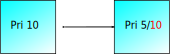
\includegraphics[scale=1.00]{images/one-to-one-inheritance}
\caption{Procesnetværk med en afsender og en modtager. Afsenderen har prioritet 10, mens modtageren har en initiel prioritet på fem. Modtageren  får via prioritetsnedarvning hævet sin prioritet til 10. (Højere er bedre)}
  \label{fig:one-to-one-inheritance}
  \end{center}
\end{figure}

\begin{figure}
 \begin{center}
  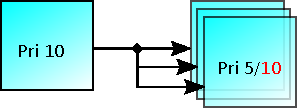
\includegraphics[scale=1.00]{images/any-to-any-inheritance}
  \caption{I dette eksempel findes der tre modtagere, som alle får hævet deres prioritet til 10.}
  \label{fig:any-to-any-inheritance}
  \end{center}
\end{figure}

Prioritetsnedarvning i et miljø med any-to-any kanaler har dermed en risiko for at medføre prioritetsdevaluering. Man kan forstille sig forskellige metoder til at eliminere eller minimere problemet f.eks ved at begrænse antallet af processer, der kan modtage en prioritetsnedarvning. Dette kunne gøres ved kun at lade en enkelt proces arve prioriteten,  men så skal man tage stilling til, hvilken proces, der skal udvælges. Dette kunne være den proces, der er tættest på at indgå i kommunikationen.  Udvælgelsen af processer må dog bero på en analyse af den enkelte applikation og dens aktuelle tilstand. Da vi ikke ønsker at begynde på en analyse af brugerens kode, må vi nødvendigvis sende prioritetsnedarvningen til alle processerne på kanalen. For at løse problemet vil vi i stedet fokusere på at minimere antallet af processer, der starter prioritetsnedarvningen, og det tidsrum processerne har arvet en prioritet.

Når kommunikationen på kanalen er gennemført, befinder processens sig i en anden tilstand og er afhængig af noget andet for at komme videre i sin udførsel. 
Når det midlertidige afhængighedsforhold ophører skal processer der har arvet en prioritet miste denne. Der skal selvfølgelig tages højde for at en proces kan arve forskellige prioriteter fra forskellige andre processer, så det skal være muligt at falde tilbage til den næsthøjeste arvede prioritet, i stedet for blot at skifte tilbage til den oprindelige prioritet. 

\subsection{Alternation}
Det er dog ikke kun i forbindelse med almindelig kommunikation vi skal forholde os til introduktionen af processer med et prioritet. I kodestrukturen \code{alternation}
 har en udvikler mulighed for at foretage et  prioriteret valg mellem flere forskellige kanaler. Et prioriteret valg mellem flere kanaler, kan dog være i konflikt med de processer som får opfyldt deres kommunikation. 
  
\citeauthor{Burns1990} beskriver og illustrerer præcist denne problemstilling i \citetitle{Burns1990}\cite{Burns1990}. Til at illustrere problemet beskriver de et eksempel, som er vist i \cref{lst:pri-select}. Denne kodestump viser et prioriteret valg mellem kanalerne A1 og A2. Til hver kanal er tilknyttet en proces, P1 og P2. Disse to processer har en prioritet tilknyttet på hhv.  Pri1 og Pri2. \CRef{tab:prioritizedSelect} viser hvilken kanal der bliver valgt, afhængig af processernes prioritet.

\begin{lstlisting}[firstnumber=1 ,float=hbtp, label=lst:pri-select, caption={(priority) select. Eksemplet er kopieret fra \cite{Burns1990}}]
(priority) select
   A1 -- Process P1
 or
   A2 -- Process P2
 end select
\end{lstlisting}

\begin{table}[htbp]
	\centering
	\begin{tabular}{lccc}
       	\toprule
                        & Pri1 > Pri2 & Pri1 = Pri2 & Pri1 < Pri2\\
        \midrule
	    priority select & A1          & A1          & ?  \\
        \bottomrule
        \end{tabular}
    \caption[]{Konflikten ved brug af prioriteret valg og procesprioriteter. Eksemplet er kopieret fra \cite[160]{Burns1990}}\\
    \label{tab:prioritizedSelect}
\end{table}

Man kan af \cref{tab:prioritizedSelect}  konstatere at der opstår en konflikt i kolonne tre, hvis udvikleren foretrækker en kanal, hvor den  tilknyttede proces' prioritet er lavere  end den anden proces'  prioritet. Man vil ikke kunne opfylde begge krav om både at kommunikere med den proces med højst prioritet, og lade udvikleren bestemme kanalen. For \citeauthor{Burns1990} er løsningen en ``orthogonal solutions'', der håndterer begge typer prioriteter. De ønsker overordnet set to typer udvælgelsesmetoder, weak- og strong Select. Weak select sorterer primært efter processernes prioritet og sekundært efter det prioriterede valg. Strong select udvælger udelukkende processer efter det prioriterede valg. De forstiller sig, at weak select skal bruges som den primære metode, men i specielle tilfælde skal en udvikler have mulighed for at tvinge et prioriteret valg igennem.

I artiklen fra \citeauthor{Burns1990} har de kun beskæftiget sig med one-to-one kanaler, og det er denne antagelse der medfører at et valg af kanal medfører et valg af en proces og dennes prioritet. Dette er ikke en mulighed i \pycsp hvor kanalerne er af typen any-to-any. Et valg af en kanal, medfører derfor ikke en direkte kobling til en proces, men til vilkårligt mange processer, der kan have individuelle  prioriteter. I \cref{sec:rtp-kommunikation} kommer vi frem til at kommunikationen altid skal sørge for at det er den højst prioriterede proces der kommunikerer. Dette kan bruges i \code{alternation} til at finde den højeste prioritet blandt de processer der er klar til at kommunikere, og bruge denne prioritet til udvælgelsen af kanal i \code{alternation}.

På baggrund af artiklen har vi valgt at \code{alternations} udfører en weak select, da denne version egner sig bedst til RTP . Vi vil i vores version ikke inkludere en strong select. Dette gør vi ud fra en betragtning om at den kun bør bruges i sjældne tilfælde,  da den vil modarbejde ideen bag RTP. Hvis en udvikler alligevel ønsker denne funktionalitet, vil har godt kunne opnå det i \pycsp, men vi ønsker ikke at tilskynde brugen, ved direkte at inkludere den.

\phantomsection
\label{misc:kanal-prioritet}
\subsubsection*{Prioritetsnedarvning i \code{alternations}}
Vi har som nævnt en klar kæde af afhængigheder i \pycsp men vi skal være opmærksomme på ikke at højne processers prioritet unødigt. Dette kan let blive tilfældet såfremt vi ikke holder ordentligt styr på, hvorfor en proces har den prioritet, den har, om den er sat af udvikleren, eller den er nedarvet. Man kan forestille sig en situation, hvor et uddrag af et proces-neværk består af en generator-forbruger-model med to generatorer og en enkelt forbruger. De to generatorer er forbundet til forbrugeren vha. en \code{alternation}, og har henholdsvis høj og lav prioritet. Eksemplet er illustreret på \cref{fig:alt-inheritance}. Forbrugeren vil i dette scenarium arve den høje prioritet fra den tilsvarende generator, men utilsigtet vil den høje prioritet derefter også propagere fra forbrugeren til generatoren med lav prioritet. Dette er ikke hensigtsmæssigt, da de to generatorer nu har lige høj prioritet og ikke det forhold, som udvikleren oprindeligt har angivet. Vi kan dog indse, at dette ikke bliver et problem, idet vi kun udfører prioritetsnedarvning i det tilfælde, hvor der ikke er nogen processer, der er er klar til at indgå i ønsket kommunikation. I det opstillede tilfælde vil forbrugeren derfor ikke foretage yderligere prioritetsnedarvning på generatoren med lav prioritet, da generatoren med høj prioritet altid vil være klar til at skrive i denne situation. 

\begin{figure}
 \begin{center}
  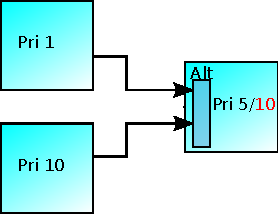
\includegraphics[scale=1.00]{images/alt-inheritance}
  \caption{Prioritetsnedarvning i \code{alternations.}}
  \label{fig:alt-inheritance}
  \end{center}
\end{figure}


\section{Design og implementation}
\fxwarning{Husk at snakke om kunstige lave prioriteter såfremt en proces arver prioritet fra flere andre processer. }
\section{Evaluering}
\section{Fremtidigt arbejde}
\section{Opsummering}
